\chapter{Planificación e Avaliación de Custes}

A planificación e a avaliación de custes son de vital importancia nun proxecto destas 
características, pois aseguran que o proxecto de desenvolverá correctamente cumprindo con todas as
especificacións desexadas. Neste caso a realización do proxecto abarca dende mediados de febreiro de
2015 cando teñen lugar as primeiras reunións ate setembro de ese mesmo ano no que finaliza a 
execución desta aplicación e a elaboración da memoria co obxectivo de presentar o conxunto do 
traballo a mediados de setembro.

Como se explicou no capítulo referente á metodoloxía, o proxecto subdividirase nunha serie de 
iteracións de aproximadamente un mes de duración\footnote{As datas non son de un mes exacto xa que
se adaptaron estes períodos en función da carga lectiva e de outras variables de carácter persoal 
para cumprir así coa faceta incremental do proxecto, facendo que cada nova Release aportase unha
serie de características de interese.}, nas que se acometerán unha serie de 
funcionalidades concretas. Para o seguimento do avance do proxecto, o seu control e avaliación 
empregase a ferramenta YouTrack, que a parte de xestionar de forma áxil as tarefas a realizar, 
permite xerar informes de proxecto como os que se verán a continuación. A parte disto, por cada 
versión estable pódese atopar no repositorio de GitHub, unha Release co seu número de versión e o 
seu comentario asociado. As Releases pódense ver na seguinte lista:

\begin{itemize}
 \item \textbf{v0.1 - Subir e Visualizar vídeos} (1 febreiro - 1 marzo) 
 \item \textbf{v0.2 - Subida y conversión de vídeo completada} (1 marzo - 19 abril)
 \item \textbf{v0.3 - Xerar e mostrar elementos básicos do XML} (19 abril - 15 maio)
 \item \textbf{v0.4 - Solventados bug's e mellorada a estratexia de probas} (15 maio - 11 xuño)
 \item \textbf{v0.5 - Traxectorias}  (11 xuño - 10 xulio)
 \item \textbf{v0.6 - Detección do comportamento anómalo} (10 xulio - 24 xulio)
 \item \textbf{v0.7 - Memoria y últimos detalles} (24 xulio - 30 agosto)
\end{itemize}

A primeira iteración do proxecto estivo principalmente centrada na formación sobre o framework
Django, xa que o fin primordial era o de crear unha primeira páxina web que permitise subir e 
visualizar vídeos. Tamén estivo centrada en coñecer de preto as posibilidades ofertadas pola
ferramenta GitHub para poder subir os avances realizados. Non se empregaba por tanto ningunha
ferramenta para o seguimento de incidencias ou a integración continua.

Durante a segunda e terceira iteración cando xa se dominaban tanto Django como GitHub, 
procedeuse á busca dunha ferramenta para este seguimento de incidencias. Nun comezo, empregouse
a propia ferramenta integrada en GitHub que permite un seguimento mínimo das tarefas e as metas
a alcanzar, e xa na terceira iteración optouse de forma definitiva por YouTrack, migrando os 
issue's acumulados en GitHub a esta nova plataforma mais completa. Durante este período tamén se
foi configurando Travis CI como servidor de integración continua, inda que a ampla diversidade
de linguaxes e tecnoloxías presentes no proxecto fixo que esta integración continua fallase 
eventualmente por motivos de configuración.

\begin{figure}[htp]
\begin{center}
    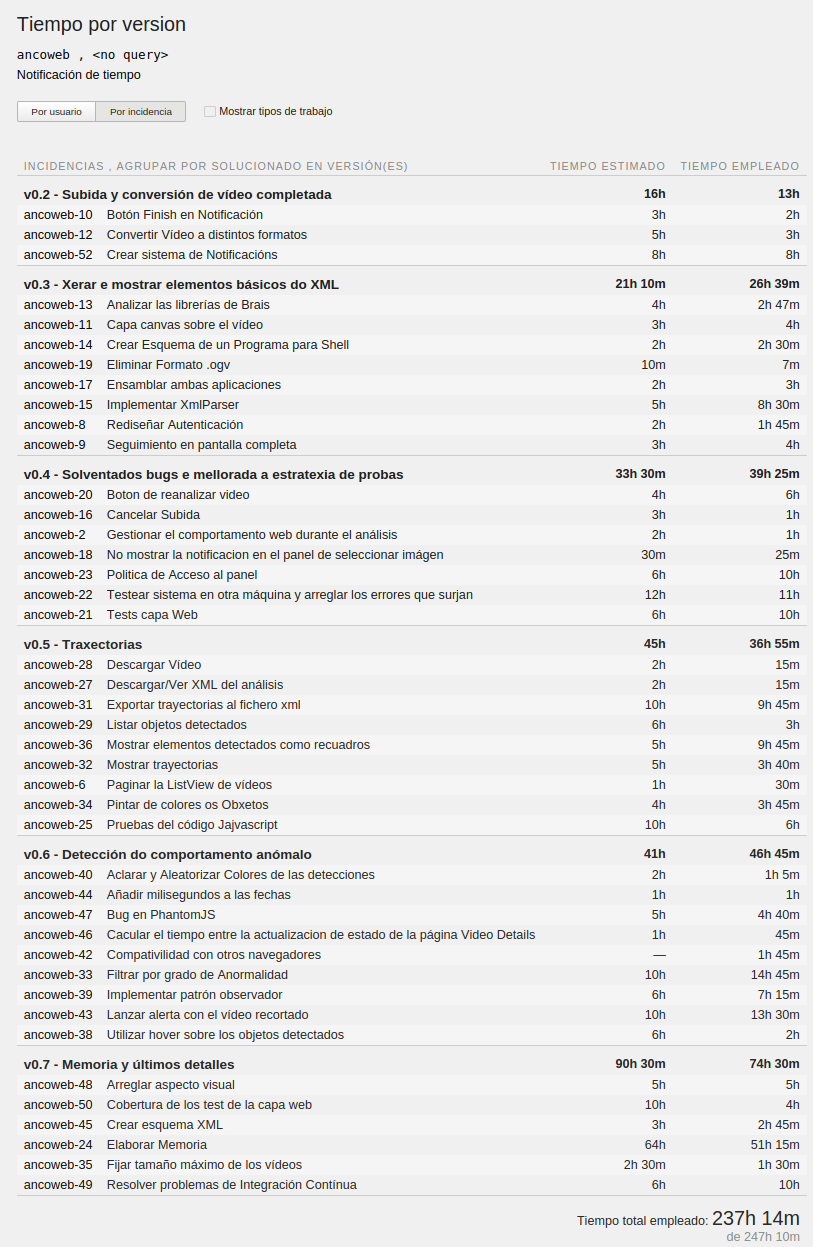
\includegraphics[scale=0.5]{figures/YouTrack/taboaCompletaHoras.png}
    \caption{Táboa completa de horas estimadas fronte a empregadas por versión}
\label{fig:taboaCompletaHoras}
\end{center}
\end{figure}

\begin{figure}[htp]
\begin{center}
    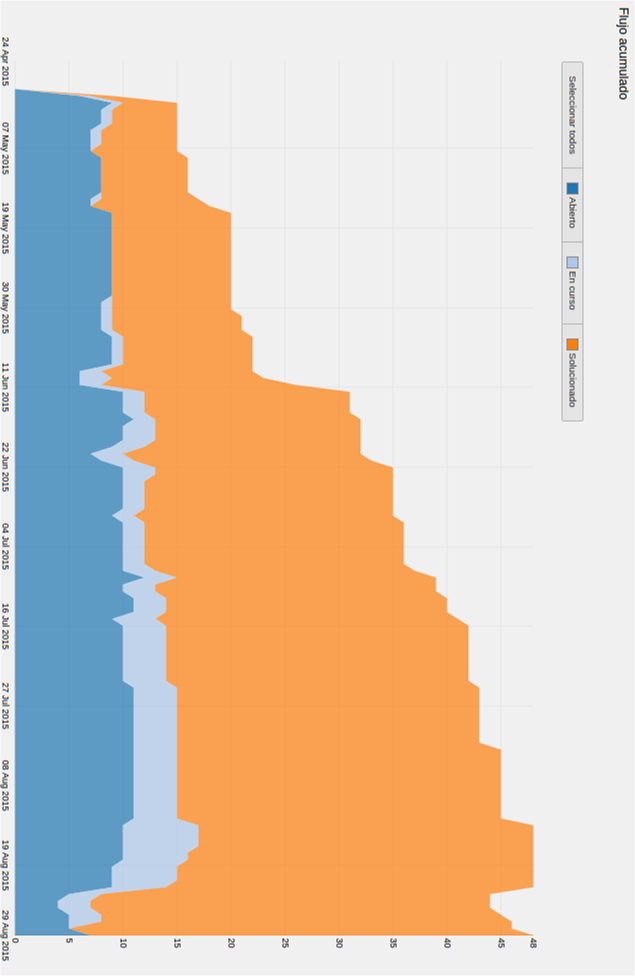
\includegraphics[scale=0.35]{figures/YouTrack/fluxoAcumulado.png}
    \caption{Gráfica do fluxo de tarefas acumulado ao longo do proxecto}
\label{fig:fluxoAcumulado}
\end{center}
\end{figure}

\begin{figure}[htp]
\begin{center}
    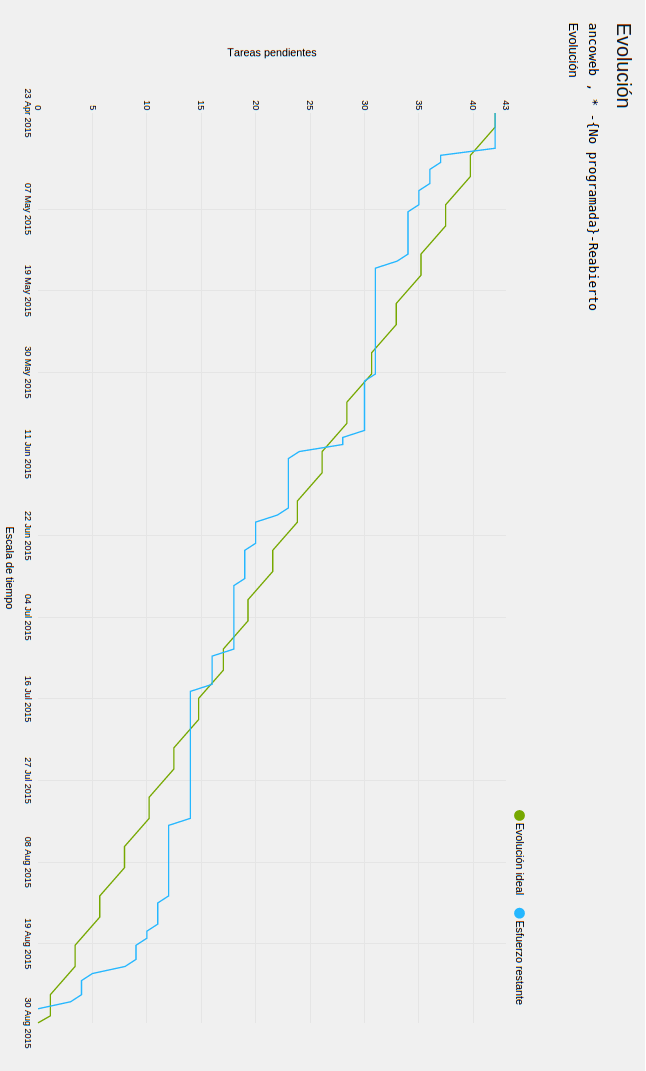
\includegraphics[scale=0.35]{figures/YouTrack/evolucionProxecto.png}
    \caption{Gráfica da evolución do proxecto}
\label{fig:fluxoAcumulado}
\end{center}
\end{figure}

Na figura \ref{fig:taboaCompletaHoras} pódense ver toda-las horas adicadas fronte ás horas
previstas, xeralmente a predición é acertada, inda que como é lóxico non é cen por cen exacta. No 
total das horas pódese ver unha gran diferencia entre as horas estimadas e as horas adicadas, isto é
así porque YouTrack contabiliza tamén as horas asignadas a tarefas que non foron estimadas, como son
a elaboración da memoria ou a comprobación en distintos navegadores.



Os datos do total de horas empregadas suman XXXXX horas, que a un prezo de 10 \euro a hora fan un custo
total de XXXXXXXXX \euro.
